Se asume que los casos de uso en los que interviene el rol de comercial pueden ser igualmente realizados por el rol de administrador, al disponer este de permisos equivalentes o superiores dentro del sistema. Por este motivo, y con el objetivo de mejorar la claridad del modelo, se ha optado por representar únicamente el rol de comercial en los casos de uso compartidos, evitando redundancias innecesarias en los diagramas. No obstante, en aquellos casos en los que existen funcionalidades exclusivas del rol de administrador, este se ha representado explícitamente.

Este enfoque es coherente con el modelado de casos de uso, en el que los actores representan roles que interactuan con el sistema \citep[Ch.~4]{sommerville}.

\bigskip

En la versión actual del proyecto, los diagramas asociados a \texttt{M1}, \texttt{M2}, \texttt{M3} y \texttt{M4} deben interpretarse como módulos ya implementados y operativos. El caso de \texttt{M5} pasa a una situación intermedia: existe ya una implementación funcional de fichas del salón, alta, edición y borrado de servicios, ficha técnica, plantillas reutilizables, sugerencias derivadas y borradores técnicos editables por servicio, pero el diagrama sigue recogiendo además capacidades aún no construidas, como el envío real del correo a cliente final. En \texttt{M6} ya existe un núcleo interno de promociones, segmentación, formaciones, notificaciones, recordatorios y descuentos promocionales aplicados al pedido, aunque la mensajería externa sigue siendo planificación futura. El diagrama de \texttt{M8} conserva valor de análisis y planificación, mientras que \texttt{M7} dispone ya de auditoría administrativa, configuración global de rate limiting, resumen operativo, integraciones de soporte, soporte técnico/PWA y un primer subsistema persistente para integraciones empresariales, operaciones de intercambio y propuestas de pedido a proveedor.

\newpage{\ }
\subsection{Casos de Uso M1.}

En este módulo se han representado los casos de uso relacionados con la gestión de acceso, alta y autorización de usuarios.

\begin{figure}[H]
    \centering
    \includegraphics[width=0.8\textwidth]{./figures/UML/CasosDeUso/M1_CasosDeUso.pdf}
    \caption{Casos de Uso M1. Gestión de acceso, alta y autorización de usuarios}
    \label{fig:M1_CasosDeUso}
\end{figure}

\newpage{\ }
\subsection{Casos de Uso M2.}

En este módulo se han representado los casos de uso relacionados con la gestión comercial y clientes.

\begin{figure}[H]
    \centering
    \includegraphics[width=0.8\textwidth]{./figures/UML/CasosDeUso/M2_CasosDeUso.pdf}
    \caption{Casos de Uso M2. Gestión comercial y clientes}
    \label{fig:M2_CasosDeUso}
\end{figure}

\newpage{\ }
\subsection{Casos de Uso M3.}

En este módulo se han representado los casos de uso relacionados con el catálogo, productos y coloración.

\begin{figure}[H]
    \centering
    \includegraphics[width=0.8\textwidth]{./figures/UML/CasosDeUso/M3_CasosDeUso.pdf}
    \caption{Casos de Uso M3. Catálogo, productos y coloración}
    \label{fig:M3_CasosDeUso}
\end{figure}

\newpage{\ }
\subsection{Casos de Uso M4.}

En este módulo se han representado los casos de uso relacionados con los pedidos, entregas y cobros.

\begin{figure}[H]
    \centering
    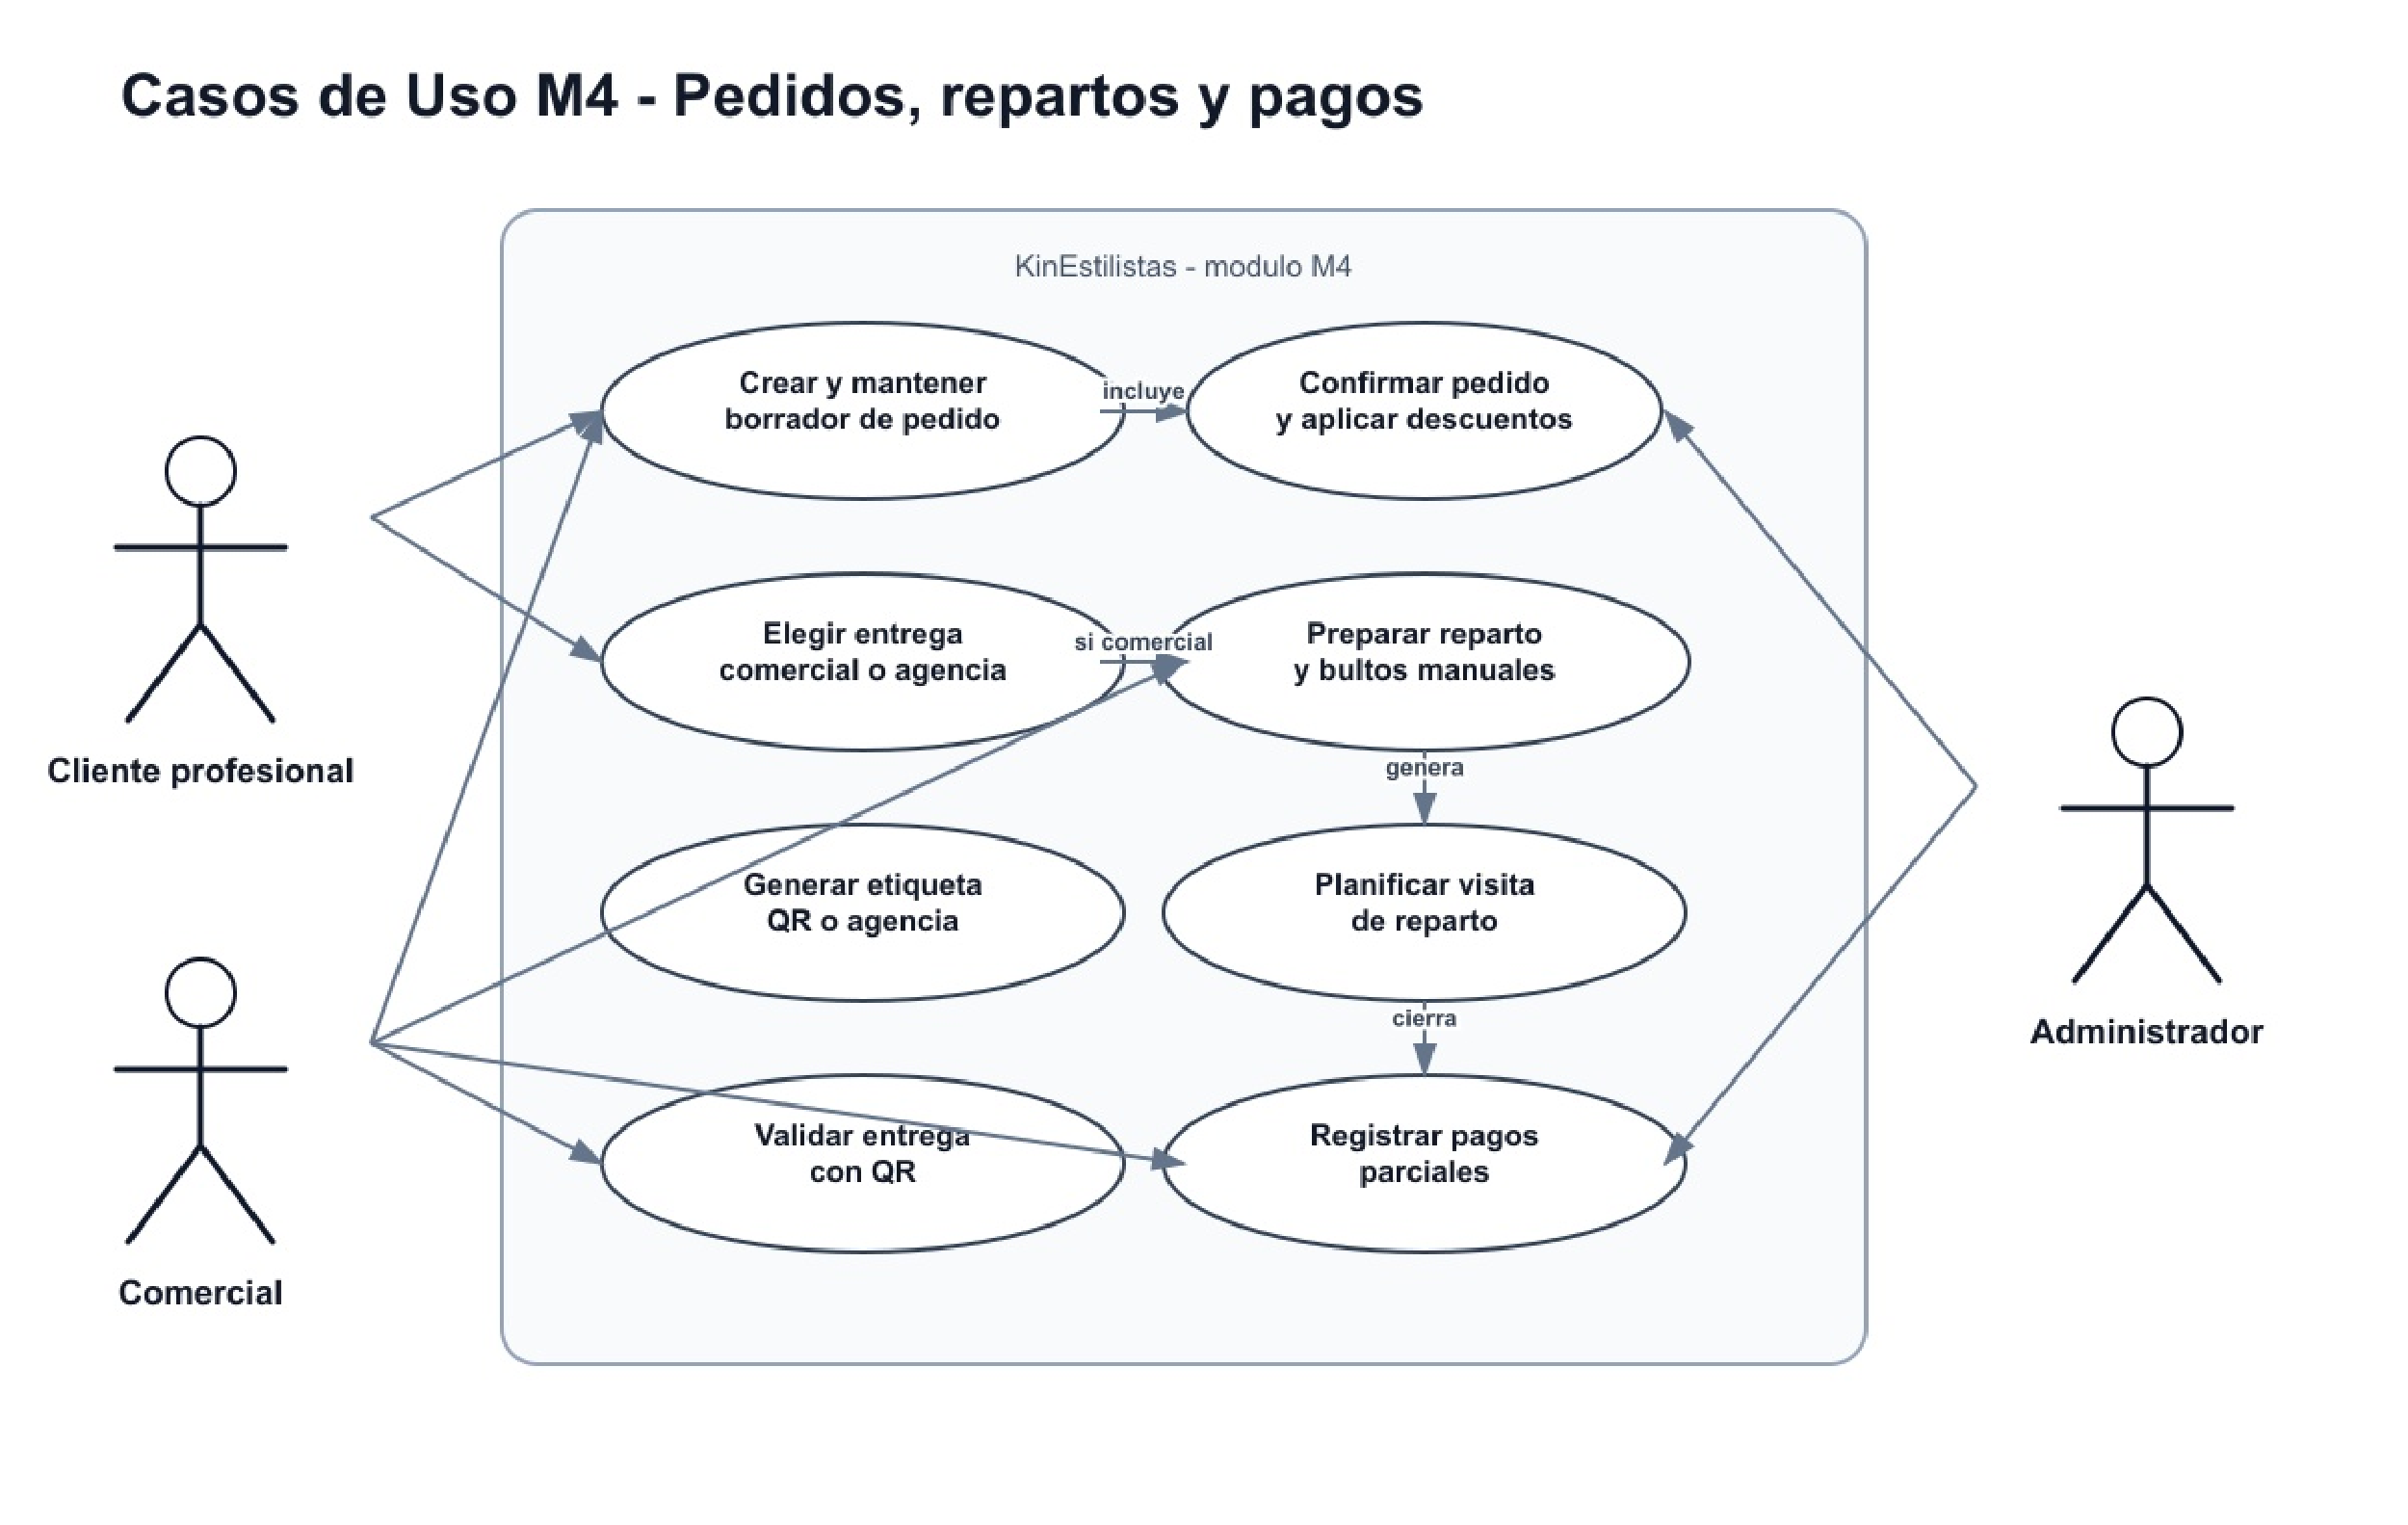
\includegraphics[width=0.8\textwidth]{./figures/UML/CasosDeUso/M4_CasosDeUso.pdf}
    \caption{Casos de Uso M4. Pedidos, entregas y cobros}
    \label{fig:M4_CasosDeUso}
\end{figure}

\newpage{\ }
\subsection{Casos de Uso M5.}

En este módulo se han representado los casos de uso relacionados con la gestión interna de peluquerías. En la implementación actual ya existe un subconjunto operativo de estos casos de uso, centrado en fichas técnicas internas, historial de servicios con mantenimiento posterior, plantillas reutilizables, uso de productos con tonalidad concreta cuando procede, galería visual del resultado final, sugerencias derivadas y preparación asistida de borradores de correo técnico.

\begin{figure}[H]
    \centering
    \includegraphics[width=0.8\textwidth]{./figures/UML/CasosDeUso/M5_CasosDeUso.pdf}
    \caption{Casos de Uso M5. Gestión interna de peluquerías}
    \label{fig:M5_CasosDeUso}
\end{figure}

\newpage{\ }
\subsection{Casos de Uso M6.}

En este módulo se han representado los casos de uso relacionados con promociones, notificaciones y formaciones. La implementación actual cubre ya el flujo interno principal: administración de promociones, segmentación manual, publicación de formaciones, notificaciones dentro de la aplicación, recordatorios personales y aplicación de descuentos promocionales sobre pedidos. Las integraciones multicanal externas siguen formando parte de la evolución futura.

\begin{figure}[H]
    \centering
    \includegraphics[width=0.8\textwidth]{./figures/UML/CasosDeUso/M6_CasosDeUso.pdf}
    \caption{Casos de Uso M6. Promociones, notificaciones y formaciones}
    \label{fig:M6_CasosDeUso}
\end{figure}

\newpage{\ }
\subsection{Casos de Uso M7.}

En este módulo se han representado los casos de uso relacionados con administración e integraciones. En la implementación real, la parte hoy desplegada de este bloque cubre auditoría, configuración global de rate limiting, resumen operativo transversal, inventario operativo de integraciones de soporte, soporte transversal a servicios externos, soporte técnico de compatibilidad/PWA, registro persistente de integraciones empresariales, operaciones de exportación o sincronización y generación de propuestas de pedido a proveedor.

\begin{figure}[H]
    \centering
    \includegraphics[width=0.8\textwidth]{./figures/UML/CasosDeUso/M7_CasosDeUso.pdf}
    \caption{Casos de Uso M7. Administración e integraciones}
    \label{fig:M7_CasosDeUso}
\end{figure}

\newpage{\ }
\subsection{Casos de Uso M8.}

En este módulo se han representado los casos de uso relacionados con funcionalidades adicionales. Dado que las funcionalidades recogidas en este módulo no forman parte del alcance principal de la versión actualmente implementada del sistema, el diagrama asociado debe interpretarse como una representación conceptual de posibles extensiones futuras de la plataforma.

\begin{figure}[H]
    \centering
    \includegraphics[width=0.8\textwidth]{./figures/UML/CasosDeUso/M8_CasosDeUso.pdf}
    \caption{Casos de Uso M8. Funcionalidades adicionales}
    \label{fig:M8_CasosDeUso}
\end{figure}
